\documentclass[aps,prl,reprint]{revtex4-2}
\usepackage{graphicx}
\usepackage[dvipsnames]{xcolor}
\usepackage{subcaption}
\usepackage{amsmath}

\definecolor{myteal}{RGB}{0,128,128}
\newcommand{\vect}[1]{\mathbf{#1}}
\newcommand{\ket}[1]{\left|#1\right\rangle}

\begin{document}

\title{Rich View Test for REVTeX}
\author{A. Author}
\email{author@example.org}
\affiliation{Department of Physics, Example University}
\date{\today}

\begin{abstract}
We test colors, figures, math macros and cross-references in the rich editor.
\end{abstract}

\maketitle

\section{Colors}
Text in \textcolor{red}{red}, \textcolor{blue}{blue}, \textcolor{ForestGreen}{ForestGreen},
\textcolor{red!50!blue}{a red--blue mix}, \textcolor{myteal}{a custom teal}, and
{\color{RoyalBlue} a whole group switched to RoyalBlue}. \colorbox{yellow}{Boxed}.

\section{Math}
The state $\ket{\psi}$ evolves with $\vect{k}\cdot\vect{r}$, see Eq.~\eqref{eq:wave}:
\begin{equation}
  \psi(\vect{r}) = e^{i \vect{k} \cdot \vect{r}}
  \label{eq:wave}
\end{equation}

\section{Figures}
Figure~\ref{fig:column} spans one column, Fig.~\ref{fig:wide} the full page,
and Fig.~\ref{fig:panels} has two panels~\cite{smith2020,doe2019}.

\begin{figure}
  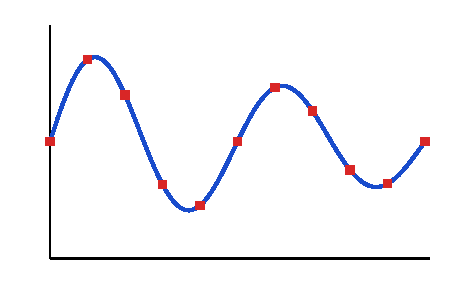
\includegraphics[width=\linewidth]{figures/curve}
  \caption{A column-width PDF figure.}
  \label{fig:column}
\end{figure}

\begin{figure*}
  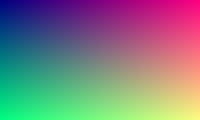
\includegraphics[width=0.8\textwidth]{figures/plot.png}
  \caption{A page-wide figure at 80\% of the text width.}
  \label{fig:wide}
\end{figure*}

\begin{figure}
  \begin{subfigure}{0.48\linewidth}
    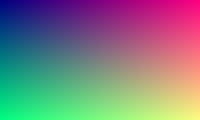
\includegraphics[width=\linewidth]{figures/plot.png}
    \caption{Left}
  \end{subfigure}\hfill
  \begin{subfigure}{0.48\linewidth}
    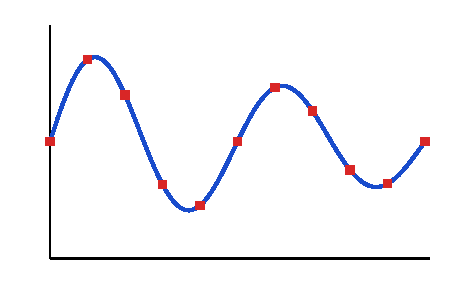
\includegraphics[width=\linewidth]{figures/curve.pdf}
    \caption{Right}
  \end{subfigure}
  \caption{Two panels.}
  \label{fig:panels}
\end{figure}

\begin{figure}
  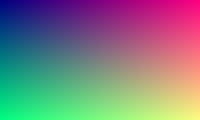
\includegraphics[scale=0.5]{figures/plot.png}
  \caption{Natural size at \texttt{scale=0.5}.}
\end{figure}

\begin{acknowledgments}
We thank the reviewers.
\end{acknowledgments}

\begin{thebibliography}{2}
\bibitem{smith2020} J. Smith, Phys. Rev. Lett. \textbf{1}, 1 (2020).
\bibitem{doe2019} J. Doe, Phys. Rev. B \textbf{2}, 2 (2019).
\end{thebibliography}

\end{document}
